\documentclass[8pt, landscape, fleqn]{scrartcl}
\setlength{\parindent}{0pt}
\usepackage[ngerman]{babel}
%\usepackage[applemac]{inputenc}
\usepackage[utf8]{inputenc}
\usepackage[dvips]{geometry}
\usepackage{latexsym}
\usepackage{multicol}
\usepackage{amsmath}
\usepackage{graphicx}
\usepackage{array}
\usepackage{booktabs}
\usepackage{amsmath}
\usepackage{mathtools}
\usepackage{ulem}
\usepackage{amsfonts}
\usepackage{dsfont}
\usepackage{charter} %%% Schreibart
%\renewcommand{\familydefault}{\sfdefault}



%%%%%%%%%%Paket für Chemische Formeln
\usepackage{chemformula} 
\usepackage[version=3]{mhchem}
%%%%%%%%%%%%%%%%% Farbe
\usepackage{color}

\pagestyle{plain}
\typearea{20}
\columnsep 30pt
\columnseprule .4pt
\setlength{\extrarowheight}{0.9em}

\renewcommand{\arraystretch}{0.8}

\makeatletter
\renewcommand{\section}{\@startsection{section}{1}{0mm}%
{-2\baselineskip}{0.8\baselineskip}%
{\hrule depth 0.2pt width\columnwidth\hrule depth1.5pt
width0.25\columnwidth\vspace*{1.2em}\Large\bfseries\rmfamily}}
\makeatother


\makeatletter
\renewcommand{\subsection}{\@startsection{subsection}{1}{0mm}%
{-2\baselineskip}{0.8\baselineskip}%
{\hrule depth 0.2pt width\columnwidth\hrule depth0.75pt
width0.25\columnwidth\vspace*{1.2em}\large\bfseries\rmfamily}}
\makeatother

\makeatletter
\renewcommand{\subsubsection}{\@startsection{subsubsection}{1}{0mm}%
{-2\baselineskip}{0.8\baselineskip}%
{\hrule depth 0.2pt width\columnwidth\vspace*{1.2em}\normalsize\bfseries\rmfamily}}
\makeatother

\newcommand{\Mx}[1]{\begin{bmatrix}#1\end{bmatrix}}
\begin{document}
\part*{\LARGE\textrm{Advanced Techniques Risk Analysis of Technical Systems $\hfill$ Xeno Meienberg}}
\begin{multicols*}{3}

\section{Introduction, Definitions \& Overview}

\textbf{Reliability}

\begin{itemize}
    \item ... is a characteristic of an item, expressed by the probability that the item performs its required function under given conditions \emph{during} a stated time interval, i.e. $(0,t]$
    \item Item = entity for investigation, i.e. component, assembly, equipment, subsystem, system 
    \item from a \textbf{qualitative} point of view, reliability is defined as the ability of an item to \textbf{remain functional}
    \item from a \textbf{quantitative} point of view, reliability is defined as the probability that \textbf{no operational interruptions} will occur during a stated time interval $R(t)$
\end{itemize}

\textbf{Availability}

\begin{itemize}
    \item Point Availability (PA) is a characteristic of an item expressed by the probability that the item performs its function \textbf{at an instant of time} $t$
    \item Qualitatively, it can be described as the dependebility 
    \item Average Availability (AA), is the expected time at which the item can perform its required function
    \item Availability is used to express Point Availability in a sloppy way or Average Availability
\end{itemize}

In comparison to Availability, the Reliability analysis includes the fact that no item is allowed to fail. This means, the function performed cannot be interrupted (redundant system however can be repaired). Availability incurs that failures can happen on the item level. \newline \newline

\textbf{Risk}

\begin{itemize}
    \item RISK = POTENTIAL DAMAGE x UNCERTAINTY
    \item Dictionary: RISK = probability of damage to a person or an object
    \item We define RISK as a function of an...
    \begin{itemize}
        \item Accident Scenario, $S$
        \item Probability, $p$
        \item Consequence, $x$
    \end{itemize}
    \item We can quantify RISK on the so-called ``Farmer's Curve'
\end{itemize}

\begin{center}
    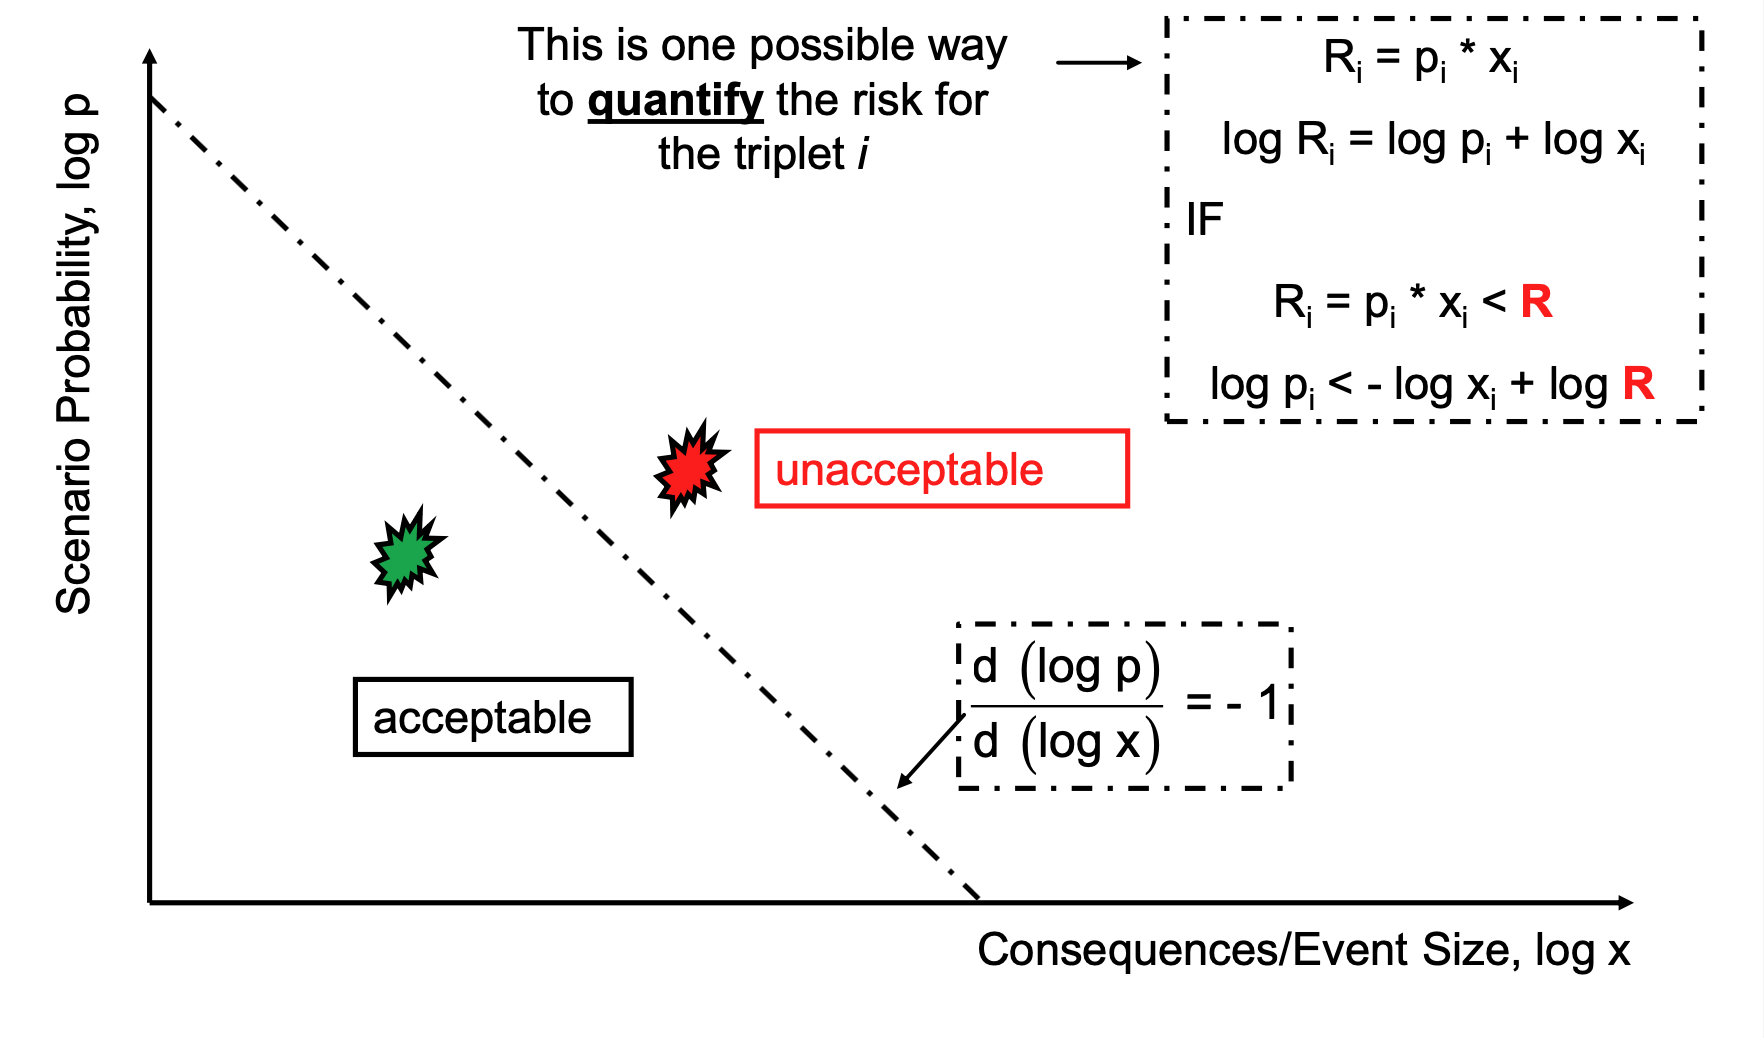
\includegraphics[width=8cm]{Images/Farmer_I.png}
    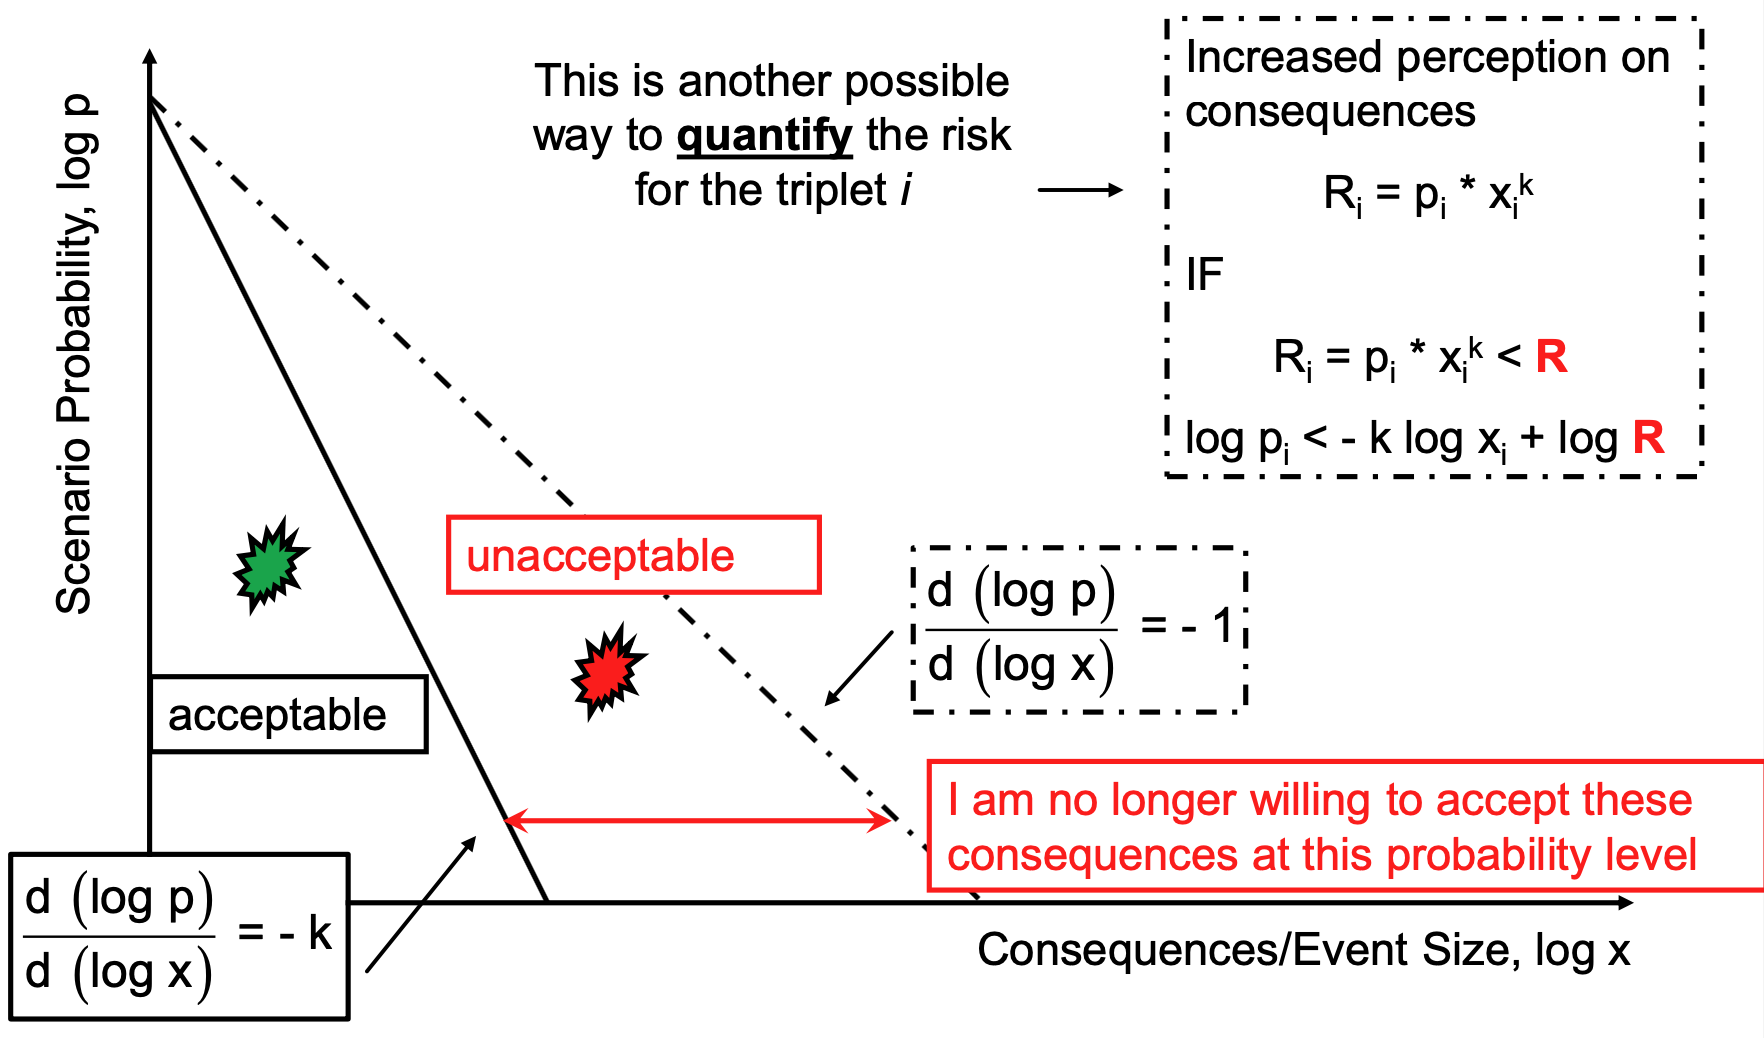
\includegraphics[width=8cm]{Images/Farmer_II.png}
\end{center}

The total Risk can be calculated as follows:

\begin{align}
    \text{Total Risk} = \sum p_i x_i^k, k\geq 1
\end{align}

It is entirely possible that the risk of different events can be dominated by either it's probability or its consequence. 

\begin{itemize}
    \item A large probability $p$ is \emph{prevented} of (minimisation based on high probability)
    \item A large consequence $x$ is \emph{mitigated, protected} (minimisation given its large impact)
\end{itemize}


\section{Probability Theory and Reliability Analysis}

Definitions:

\begin{itemize}
    \item Experiment $\epsilon$
    \item Sample space $\Omega$
    \item Event $E$
\end{itemize}

An event $E$ is a subset of the sample space $\Omega$ and the experiment $\varepsilon$ yields a set of possible outcoms ($= E$) of the experiment  \newline \newline \emph{Certain Events} follow \emph{Boolean Logic}, an event $E$ can occur or not occur, meaning an \emph{Indicator Variable} $X_E$ is 0 when $E$ does not occur and 1 if $E$ occurs \newline \newline
\emph{Uncertain Events} follow can either be true or false, with each a probability associated to it. Event $E$ in sample space $\Omega$ is triggered with a probability that the outcome has happened or not 

\subsubsection*{Classical Probability}

\begin{itemize}
    \item The experiment $\epsilon$ has $N$ possible, elementary, mutually exclusive and equally probable outcomes $A_1, A_2,..., A_N \in \Omega$
    \item The event $E = A_1 \cup A_2 \cup ... \cup A_M$,  $M\leq N$
    \item The probability of event $E$ is defined as $p(E) = M / N$
\end{itemize}

\subsubsection*{Kolmogorov Axioms}

\begin{enumerate}
    \item $0 \leq P(E) \leq 1$
    \item $P(\Omega) = 1$, $P(\emptyset) = 0$
    \item Mutually exclusive events: $P(\cup_i E_i) = \sum p(E_i)$
    \item Non-mutually exlusive events: \newline $P(A\cup B) = P_A + P_B - P(A \cap B)$
    \item Conditional probability: $P(A|B) = P(A\cap B) / P(B)$
    \item Theorem of total probability: Given an event $A$ in $\Omega$ where the space is consisting of exclusive and exhaustive events $\cup_j E_j = \Omega$: $P(A) = \Sigma_i(P(A | E_i)P(E_i))$
\end{enumerate}

\subsubsection*{Random Variables}

\begin{itemize}
    \item \textbf{CDF}: Is a non-decreasing function and returns the probabilty (state) from random variable $X$ from $0$ to a given point $A$: $F_X(X = A) = P(0 < X \leq A)$ 
    \item \textbf{pdf}: Probability of per unit $x$ (continuous)
    \item \textbf{pmf}: Histogram, it assignes the probability to discrete values $x$
\end{itemize}

\subsubsection*{Summary}

\begin{itemize}
    \item Distribution Percentile $x_\alpha$:
    \begin{itemize}
        \item $F_X(x_\alpha) = \alpha / 100 = \int_{-\infty}^{x_\alpha} f_X(x)dx$
    \end{itemize}
    \item Median:
    \begin{itemize}
        \item $F_X(x_50) = 0.5$
    \end{itemize}
    \item Mean:
    \begin{itemize}
        \item $\mu_X = E[X] = <X> = \sum_i x_i p_i$ (discrete)
        \item $= \int_{-\infty}^{\infty} x f_X(x) dx$ (continuous)
    \end{itemize}
    \item Variance:
    \begin{itemize}
        \item $\sigma_X^2 = \sum(x_i - \mu_X)^2 p_i$ (discrete)
        \item $ = \int_{-\infty}^\infty (x-\mu_X)^2 f_X(x) dx$ (continuous)
    \end{itemize}
\end{itemize}

\subsubsection*{Hazard Function (Failure Rate)}

 For risk and reliability analyses, we can use models whereas the time to failure of a component T can be expressed through a CDF $F_T(t)$ and a pdf $f_T(t)$. The complementary, cumulative function is 
 
 \begin{equation}
    R(t) = 1-F_T(t) = P(T\geq t)
 \end{equation}   

 which is decribed as the \textbf{Reliability or Survival Function} of the component T at time t and gives the probability of it surviving up to time t without failures. \newline 

 In order to monitor the failure evolution, given the component has survived up to time $t$ in a time interval $dt$, one can define a so called \textbf{Hazard Function or Failure Rate} $h_T(t)$. 

 \begin{equation}
     h_T(t) dt = P(t< T \leq t + dt | T>t) = \frac{P(t<T \leq t+t+dt)}{P(T>t)} = \frac{f_T(t)dt}{R(t)}
 \end{equation}

 The hazard function is depending on time, and is often discribed through the bathtub curve. The failure rate at the beginning is higher (infant mortality, burn in) and decreses after a certain time. The failure rate becomes constant $\lambda$ and increases at the end through ageing. 

 \begin{center}
     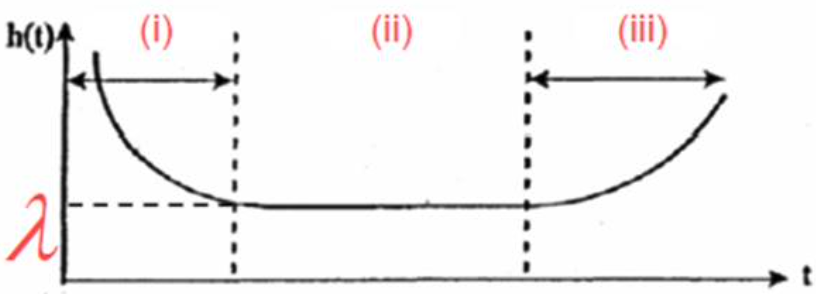
\includegraphics[width=6cm]{Images/Hazard_Function.png}
 \end{center}

 Through the definition of $R(t)$ and integrating the hazard function, we receive:

 \begin{align}
     F_T(t) = 1-e^{-\int_0^t h_T(\tilde{t}) d\tilde{t}} \\
     R(t) = e^{-\int_0^t h_T(\tilde{t}) d\tilde{t}}
 \end{align}

 If our hazard function is in its constant phase (constant hazard rate), the failure evolution follows the \textbf{Exponential Distribution}:

 \begin{align}
    h_T(t) \lambda, t>0 \\
     F_T(t) = P(T \leq t) = 1-e^{-\lambda t} \\
     R(t) = \begin{dcases}
         f_T(t) = \lambda e^{-\lambda t} & t \geq 0 \\
        0 & t < 0
     \end{dcases}
 \end{align}

 \begin{center}
     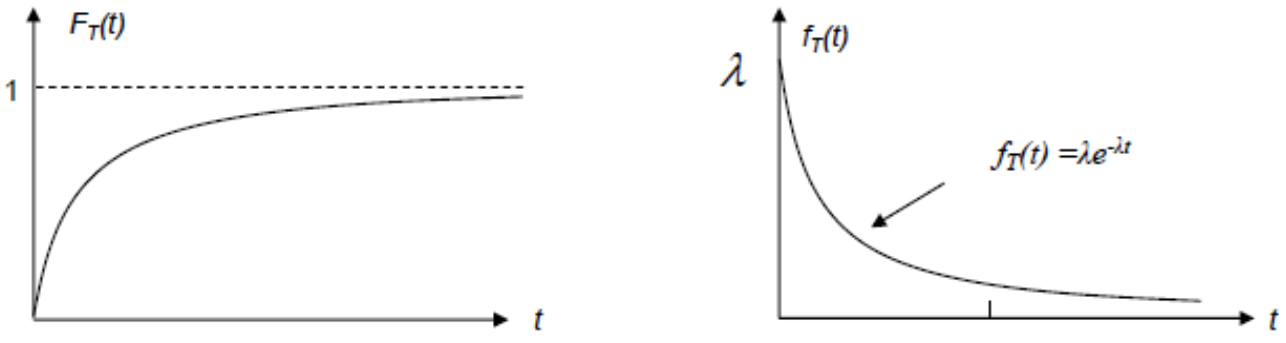
\includegraphics[width = 8cm]{Images/Exponential_Distribution.png}
 \end{center}

 The mean time to failure (MTTF) can be found through the expectation value

 \begin{align}
     E[T] = \frac{1}{\lambda} = MTTF \\
     Var[T] = \frac{1}{\lambda^2}
 \end{align}

 The failure process is memoryless. Given a component has survived at least until time $t_1$, the probability of it failing between time $t_1$ and $t_2$ is only depending on the time inbetween and not prior to time $t_1$

 \begin{align}
     P(t_1 < T < t_2) = \frac{P(t_1 < T < t_2)}{P(T > t_1)} = \frac{F_T(t_2)-F_T(t_1)}{1-F_T(t_1)} = \\
     \frac{e^{-\lambda t_1}-e^{-\lambda t_2}}{e^{-\lambda t_1}} = 1-e^{-\lambda(t_2-t_1)}
 \end{align}

The influence of an ageing process of the components failure rate shows that is not constant through time and hence can be described through the Weibull distribution. 

\subsubsection*{Boolean Logic - Fault Tree Analysis}



\subsubsection*{Minimal Cut Sets}


\end{multicols*}
\end{document}

